\section{Methodology}

% System Block Diagram
% model design architecture
% Dataset Preparation Block Diagram
% Dataset Visualization
% Box Plot of Dataset Distribution
% Model Design Stucture
% Trainable parameters
% Evaluation Metrices
% Instrumentation

% Result Slide


% slides for Remaining Workks


\methodologyslide{t}{
    System Block Diagram
}{
    \begin{figure}[!htbp]
        \centering
        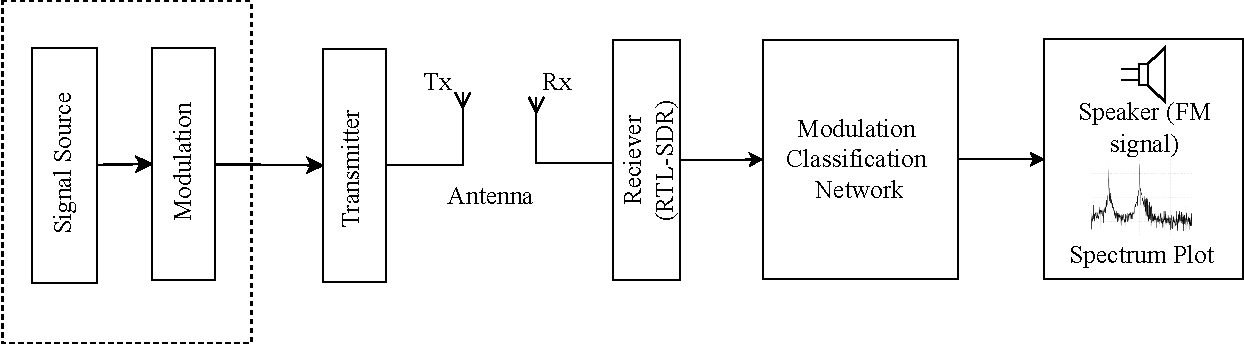
\includegraphics[width=0.9\linewidth]{img/drawio/vectors/System.pdf}
    \end{figure}
}


\methodologyslide{t}{
    Flow Diagram of Model Design
}{
    \begin{figure}[!htbp]
        \centering
        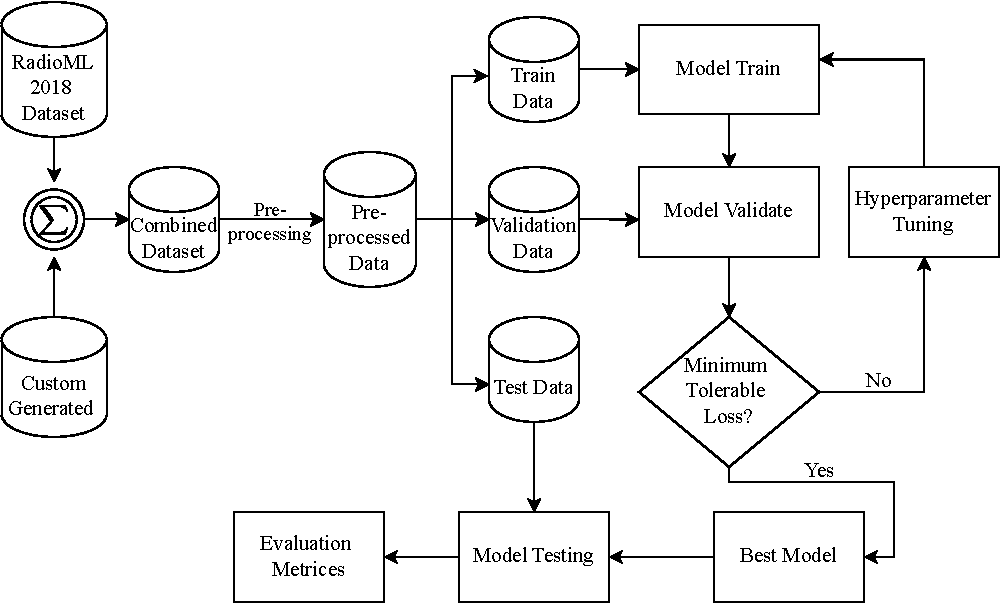
\includegraphics[width=1.1\textheight]{img/drawio/vectors/FlowDiagramOfSystemDesign.pdf}
    \end{figure}
}


% Dataset Description
\methodologyslide{t}{
    Dataset Generation Pipeline
}{
    \begin{figure}[!htbp]
        \centering
        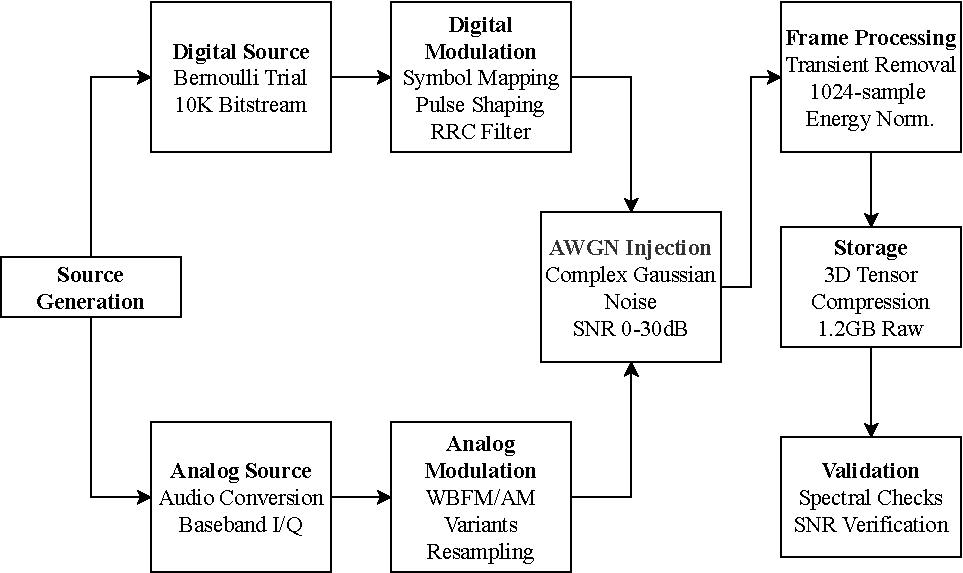
\includegraphics[width=1.2\textheight]{img/drawio/vectors/DatasetGeneration.pdf}
    \end{figure}
}

  
% Pre-processing Pipeline Slide
\methodologyslide{t}{Pre-processing Pipeline}{
    \begin{figure}
        \centering
        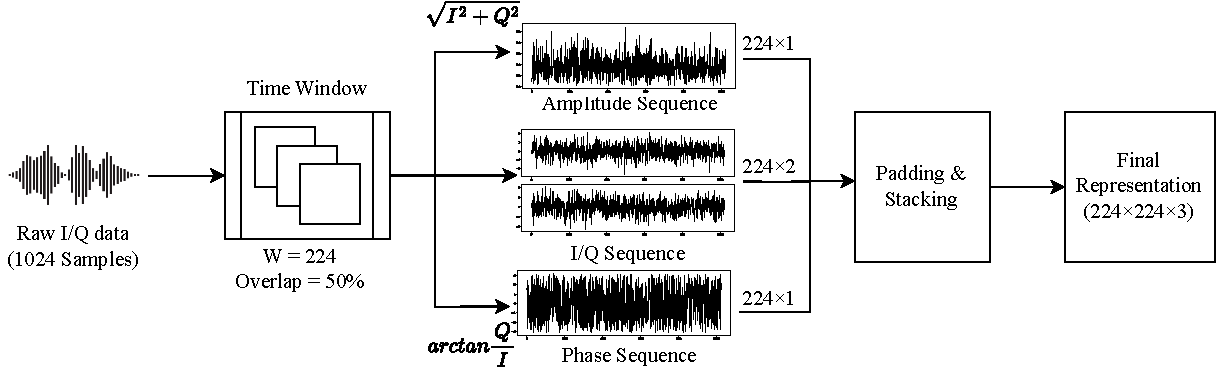
\includegraphics[width=\linewidth]{img/drawio/vectors/preprocessing.pdf}
    \end{figure}
}

\methodologyslide{t}{Preprocessed Output}{
    \begin{figure}
        \centering
        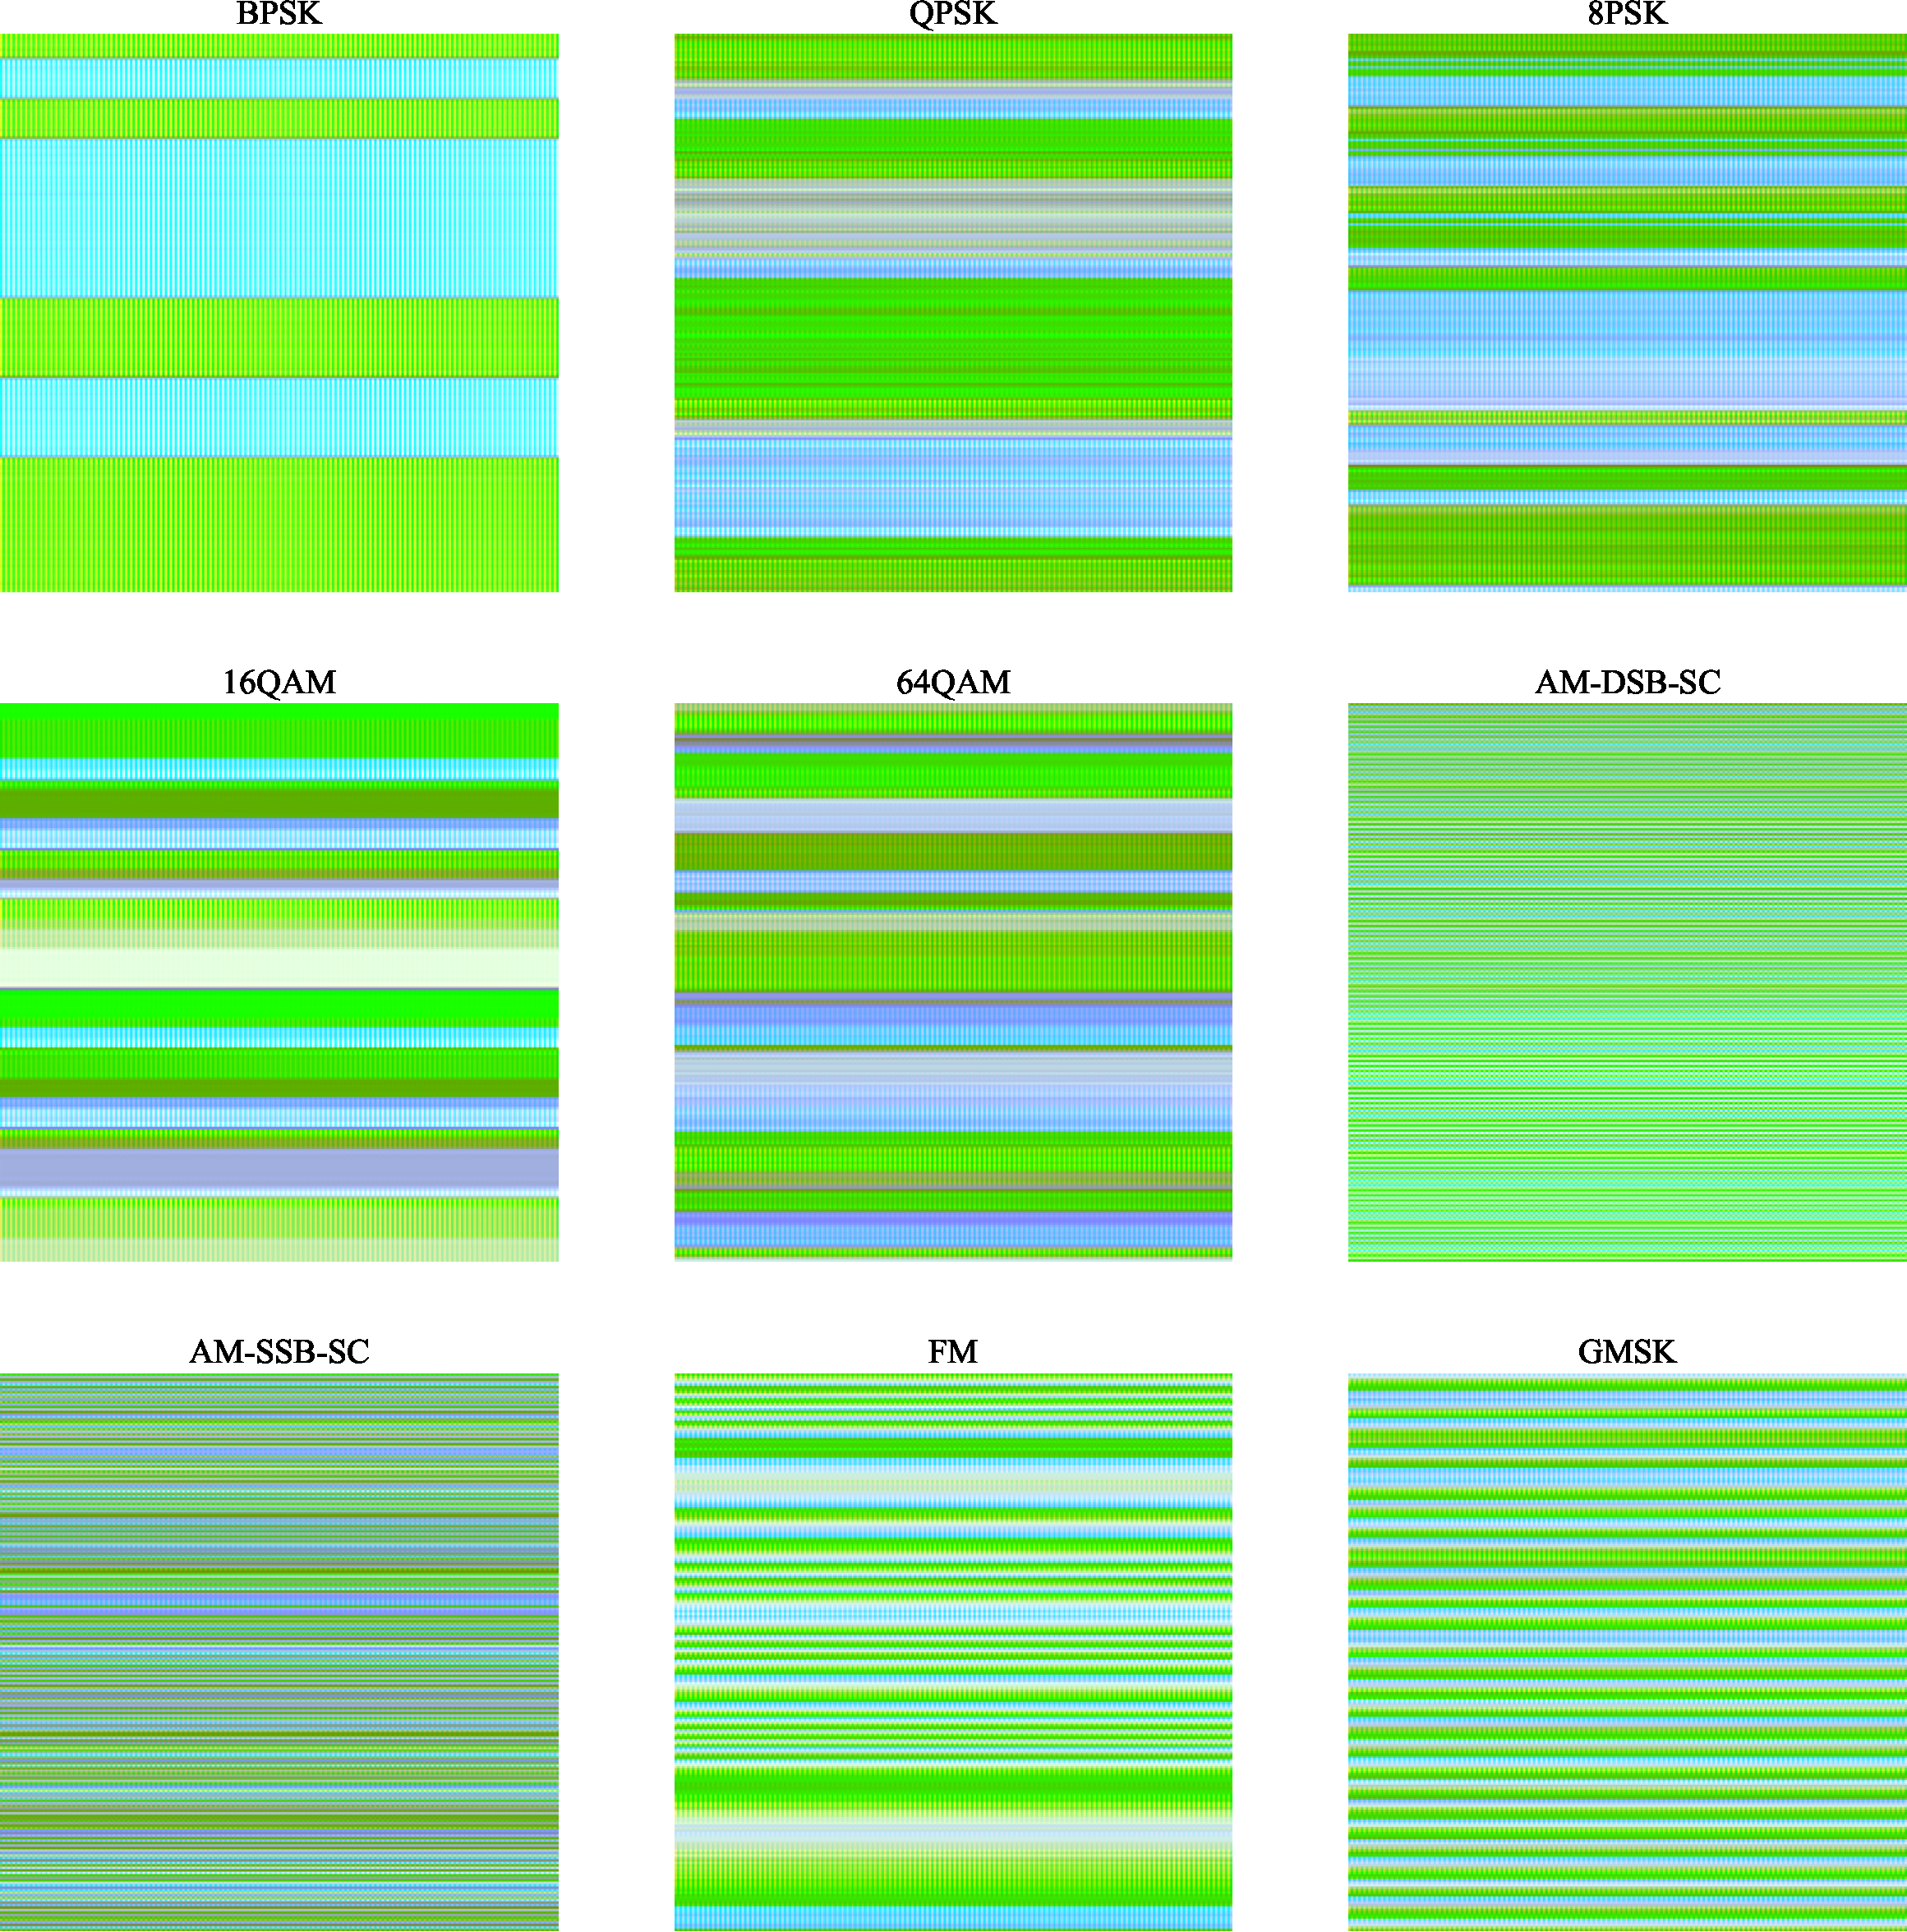
\includegraphics[width=0.35\linewidth]{img/impl/preprocessed_image.pdf}
    \end{figure}
}
% Model Architecture Slide
\methodologyslide{t}{Model Architecture}{
    \begin{figure}
        \centering
        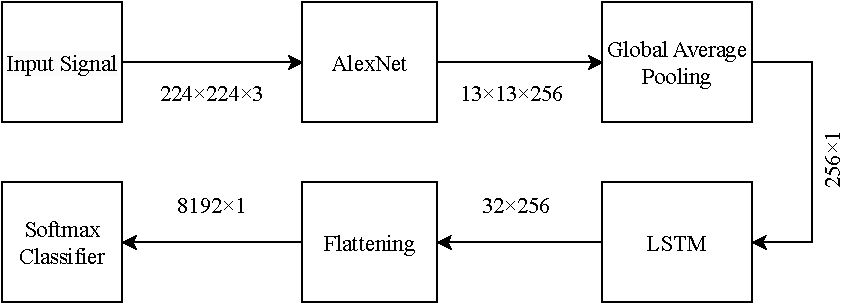
\includegraphics[width=\textwidth]{img/drawio/vectors/mod_architecture.pdf}
    \end{figure}
}

\methodologyslide{t}{AlexNet Architecture}{
    \begin{figure}
        \centering
        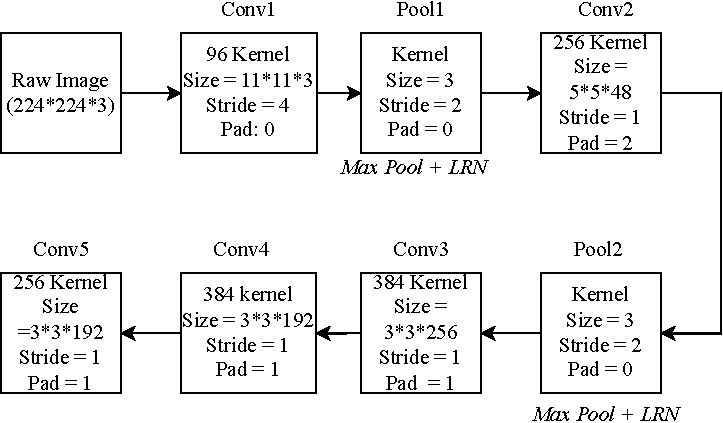
\includegraphics[scale=0.89]{img/drawio/vectors/AlexNet.pdf}
    \end{figure}
}

\methodologyslide{t}{LSTM Architecture}{
    \begin{figure}
        \centering
        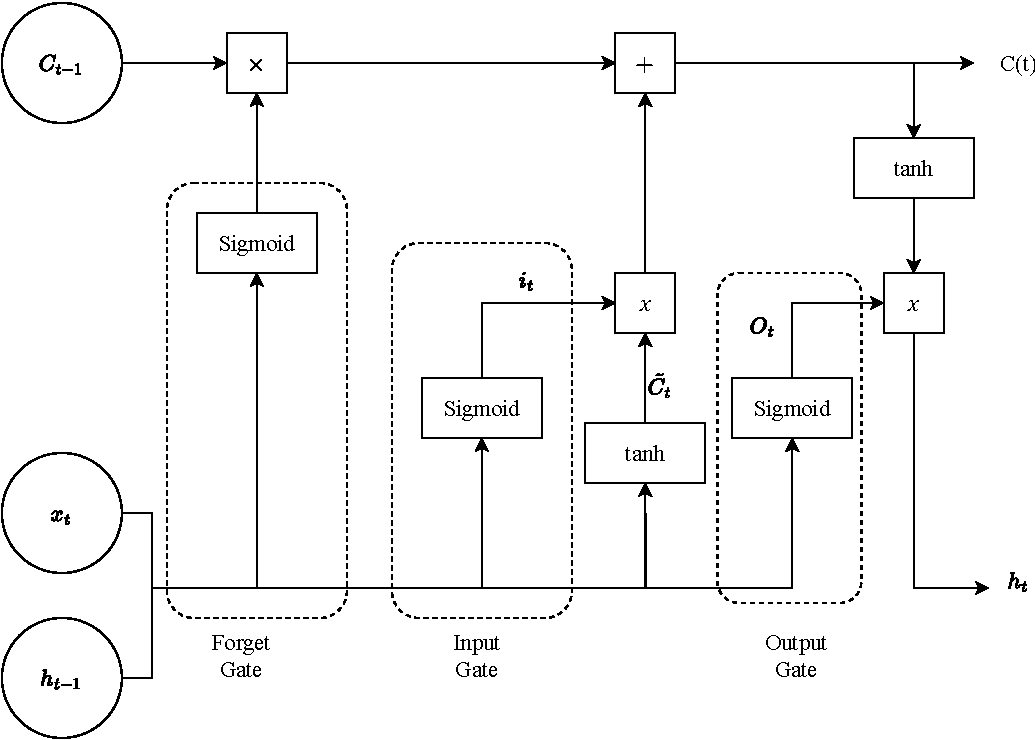
\includegraphics[scale=0.49]{img/drawio/vectors/lstm_architecture.pdf}
    \end{figure}
}

\methodologyslide{t}{Softmax Classifier}{
    \begin{figure}
        \centering
        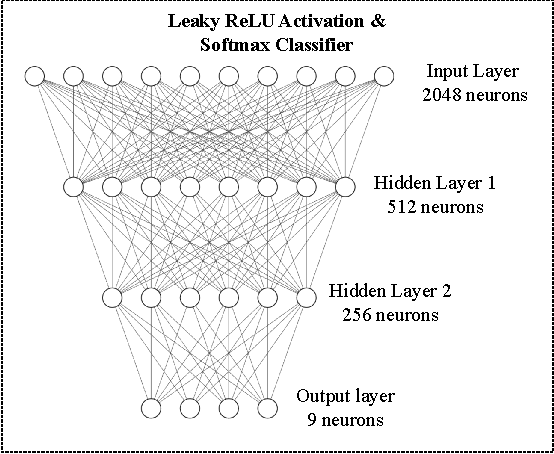
\includegraphics[scale=0.75]{img/drawio/vectors/fully_connected_layer.pdf}
    \end{figure}
}


\methodologyslide{t}{Trainable Parameters}{
    \textbf{\large AlexNet}
    \begin{table}[h!]
        \centering
        \resizebox{0.8\textwidth}{!}{%
        \begin{tabular}{lcccc}
            \toprule
            \textbf{Layer} & \textbf{Kernel Size} & \textbf{Stride} & \textbf{Padding} & \textbf{Parameters} \\
            \midrule
            Conv1 & 11$\times$11 & 4 & 2 & 34,944 \\
            Conv2 & 5$\times$5   & 1 & 2 &  614,656 \\
            Conv3 & 3$\times$3   & 1 & 1 & 885,120 \\
            Conv4 & 3$\times$3   & 1 & 1 &  1,327,488 \\
            Conv5 & 3$\times$3   & 1 & 1 &  884,392 \\
            \midrule
            \textbf{Total} & & & & 3,746,600 \\
            \bottomrule
        \end{tabular}
        }
    \end{table}
}


\methodologyslide{t}{Trainable Parameters}{
    \textbf{\large LSTM}
    \begin{itemize}
        \item Input size: 256 features per time step
        \item Hidden size: 256 units in hidden state
        \item 4 weight matrices for input, forget, cell, and output gates
        \item Weights for each gate: \( 256 \times 256 \)
        \item Biases: 4 vectors of size 256
        \item Total parameters: 525,312
    \end{itemize}
}


\methodologyslide{t}{Trainable Parameters}{
    \textbf{\large Fully Connected Layer}
    \\[2em]
    \begin{table}[h!]
        \centering
        \small
        \begin{tabular}{lcccc}
            \toprule
            \textbf{Layer} & \textbf{Neurons} & \textbf{Weights} & \textbf{Biases} & \textbf{Total} \\
            \midrule
            Input Layer - Hidden Layer 1 & 2048 - 512 & 2048$\times$512 & 512 & 1,049,088 \\
            Hidden Layer 1 - 2 & 512 - 256   & 512$\times$256 & 256 &  131,328 \\
            Hidden Layer 2 - Output Layer & 256 - 11   & 256$\times$11 & 11 & 2,827 \\
            \midrule
            \textbf{Total} & & & & \textbf{1,183,243} \\
            \bottomrule
        \end{tabular}
    \end{table}
}

\methodologyslide{t}{Total Trainable Parameters}{
    \begin{itemize}
        \item \textbf{AlexNet:} 3,746,600 parameters \vfill
        \item \textbf{LSTM:} 525,312 parameters \vfill
        \item \textbf{Fully Connected Layer:} 1,183,243 parameters \vfill
        \item \textbf{Total:} 5,455,155 parameters \vfill
    \end{itemize}
}

\methodologyslide{t}{FM Transmitter}{
    \begin{figure}
        \centering
        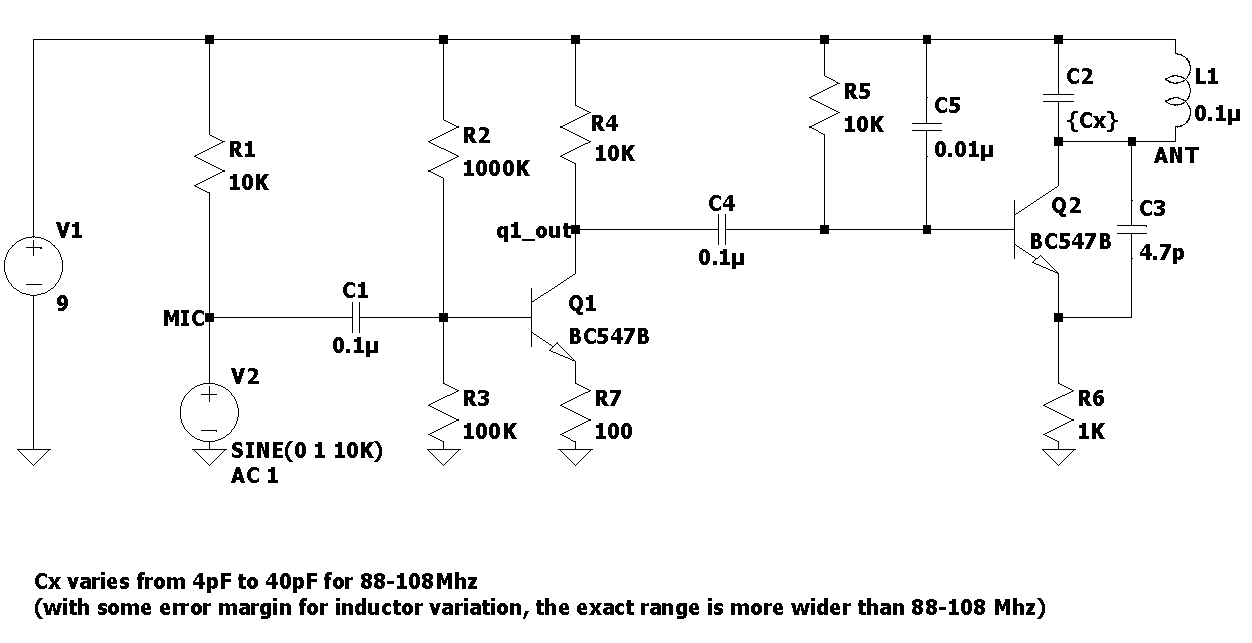
\includegraphics[scale=0.6]{img/ch4/transmitter_sch.pdf}
    \end{figure}
}

% % Slide 2: Precision
% \methodologyslide{t}{Evaluation Metrics}{
%   \textbf{\large Precision}
%   \begin{itemize}
%       \item Precision measures correctly predicted positive instances among all predicted positives. \\[1em]
%       \item Formula for each class: \\[2em]
%       \begin{equation}
%           \text{Precision}_i = \frac{\text{TP}_i}{\text{TP}_i + \text{FP}_i}
%       \end{equation}
%       \item Macro and weighted averaging methods for multiclass problems.
%   \end{itemize}
% }

% % Slide 3: Recall
% \methodologyslide{t}{Evaluation Metrics}{
%   \textbf{\large Recall}
%   \begin{itemize}
%       \item Recall (Sensitivity) measures actual positives correctly identified. \\[1em]
%       \item Formula for each class: \\[1em]
%       \begin{equation}
%           \text{Recall}_i = \frac{\text{TP}_i}{\text{TP}_i + \text{FN}_i}
%       \end{equation}
%   \end{itemize}
% }

% % Slide 4: F1 Score
% \methodologyslide{t}{Evaluation Metrics}{
%   \textbf{\large F1 Score}
%   \begin{itemize}
%       \item F1 Score is the harmonic mean of Precision and Recall. \\[1em]
%       \item Formula for each class: \\[1em]
%       \begin{equation}
%           \text{F1 Score}_i = 2 \times \frac{\text{Precision}_i \times \text{Recall}_i}{\text{Precision}_i + \text{Recall}_i}
%       \end{equation} \\[1em]
%       \item Macro and weighted averaging methods.
%   \end{itemize}
% }

% % Slide 5: Accuracy
% \methodologyslide{t}{Evaluation Metrics}{
%   \textbf{\large Accuracy}
%   \begin{itemize}
%       \item Accuracy is the proportion of correct predictions out of all predictions. \\[1em]
%       \item Formula: \\[1em]
%       \begin{equation}
%           \text{Accuracy} = \frac{\sum_{i=1}^{N} \text{TP}_i + \text{TN}_i}{\sum_{i=1}^{N} \text{Total Predictions}_i}
%       \end{equation}
%   \end{itemize}
% }

% % Slide 6: Confusion Matrix
% \methodologyslide{t}{Evaluation Metrics}{
%   \textbf{\large Confusion Matrix}
%   \begin{itemize}
%       \item A square matrix showing true vs. predicted classifications. \\[1em]
%       \item For multiclass classification \\[1em]
%       \begin{itemize}
%           \item \(C_{ij}\): Instances of class \(i\) predicted as class \(j\).
%           \item Diagonal: True Positives.
%           \item Off-diagonal: Misclassifications.
%       \end{itemize} 
%   \end{itemize}
% }

% % Slide 7: AUC-ROC
% \methodologyslide{t}{Evaluation Metrics}{
%   \textbf{\large AUC-ROC}
%   \begin{itemize}
%       \item Measures the ability of the model to distinguish between classes. \\[1em]
%       \item For each class (One-vs-Rest): \\[1em]
%       \begin{equation}
%           \text{TPR}_i = \frac{\text{TP}_i}{\text{TP}_i + \text{FN}_i}, \quad \text{FPR}_i = \frac{\text{FP}_i}{\text{FP}_i + \text{TN}_i}
%       \end{equation} \\[1em]
%       \item AUC is the area under the ROC curve.
%   \end{itemize}
% }

% % Slide 8: Top-k Accuracy
% \methodologyslide{t}{Evaluation Metrics}{
%   \textbf{\large Top-k Accuracy}
%   \begin{itemize}
%       \item Useful for problems with overlapping classes. \\[1em]
%       \item Formula: \\[1em]
%       \begin{equation}
%           \text{Top-}k\text{ Accuracy} = \frac{\text{Number of Correct Predictions in Top-}k}{\text{Total Predictions}}
%       \end{equation}
%   \end{itemize}
% }

% Frame for GPU and RTL-SDR
\methodologyslide{t}{Instrumentation}{
  \begin{itemize}
      \item \textbf{GPU (Graphics Processing Units):}
      \begin{itemize}
          \item Essential for handling computational complexity in Neural Networks.
          \item Real-time processing achieved through parallelism of GPUs. \\[1em]
      \end{itemize} 
      \item \textbf{RTL-SDR}
      \begin{itemize}
          \item Cost-effective tool for capturing RF frequencies (500 kHz - 1.75 GHz).
          \item Provides raw I/Q samples for amplitude and phase extraction.
          \item Ideal for real-time signal processing with tools like GNU Radio.
      \end{itemize}
  \end{itemize}
}

% Frame for MATLAB & Communication Toolbox, and GNU Radio
\methodologyslide{t}{Instrumentation}{
  \begin{itemize}
      \item \textbf{GNU Radio:}
      \begin{itemize}
          \item Open-source signal processing toolkit for SDR.
          \item Enables RF transmission, reception, and preprocessing.
          \item Supports real-time data acquisition with RTL-SDR hardware. \\[1em]
      \end{itemize}
      \item \textbf{PyQt6}
      \begin{itemize}
          \item Used for GUI Development of Signal Visualizer
          \item Provides a set of Python bindings for the Qt application framework.
      \end{itemize}
  \end{itemize}
}

% Frame for PyTorch and Other Software Tools
\methodologyslide{t}{Instrumentation}{
  \begin{itemize}
      \item \textbf{PyTorch:}
      \begin{itemize}
          \item Builds the CNN-LSTM hybrid architecture for AMC.
          \item Facilitates model training, validation, and deployment.
          \item Supports dataset preparation and performance evaluation. \\[1em]
      \end{itemize}
      \item \textbf{Other Software Tools:}
      \begin{itemize}
          \item \textbf{LTSpice:} FM transmitter circuit simulation
          \item \textbf{Matplotlib:} Visualization of signals and training metrics
          \item \textbf{Scikit-learn:} Data preprocessing and baseline classifier evaluation
      \end{itemize}
  \end{itemize}
}